\documentclass[journal,12pt,twocolumn]{IEEEtran}
\usepackage{setspace}
\usepackage{gensymb}
\usepackage{caption}
%\usepackage{multirow}
%\usepackage{multicolumn}
%\usepackage{subcaption}
%\doublespacing
\singlespacing
\usepackage{csvsimple}
\usepackage{amsmath}
\usepackage{multicol}
%\usepackage{enumerate}
\usepackage{amssymb}
%\usepackage{graphicx}
\usepackage{newfloat}
%\usepackage{syntax}
\usepackage{listings}
\usepackage{iithtlc}
\usepackage{color}
\usepackage{tikz}
\usetikzlibrary{shapes,arrows}



%\usepackage{graphicx}
%\usepackage{amssymb}
%\usepackage{relsize}
%\usepackage[cmex10]{amsmath}
%\usepackage{mathtools}
%\usepackage{amsthm}
%\interdisplaylinepenalty=2500
%\savesymbol{iint}
%\usepackage{txfonts}
%\restoresymbol{TXF}{iint}
%\usepackage{wasysym}
\usepackage{amsthm}
\usepackage{mathrsfs}
\usepackage{txfonts}
\usepackage{stfloats}
\usepackage{cite}
\usepackage{cases}
\usepackage{mathtools}
\usepackage{caption}
\usepackage{enumerate}	
\usepackage{enumitem}
\usepackage{amsmath}
%\usepackage{xtab}
\usepackage{longtable}
\usepackage{multirow}
%\usepackage{algorithm}
%\usepackage{algpseudocode}
\usepackage{enumitem}
\usepackage{mathtools}
\usepackage{hyperref}
%\usepackage[framemethod=tikz]{mdframed}
\usepackage{listings}
    %\usepackage[latin1]{inputenc}                                 %%
    \usepackage{color}                                            %%
    \usepackage{array}                                            %%
    \usepackage{longtable}                                        %%
    \usepackage{calc}                                             %%
    \usepackage{multirow}                                         %%
    \usepackage{hhline}                                           %%
    \usepackage{ifthen}                                           %%
  %optionally (for landscape tables embedded in another document): %%
    \usepackage{lscape}     


\usepackage{url}
\def\UrlBreaks{\do\/\do-}


%\usepackage{stmaryrd}


%\usepackage{wasysym}
%\newcounter{MYtempeqncnt}
\DeclareMathOperator*{\Res}{Res}
%\renewcommand{\baselinestretch}{2}
\renewcommand\thesection{\arabic{section}}
\renewcommand\thesubsection{\thesection.\arabic{subsection}}
\renewcommand\thesubsubsection{\thesubsection.\arabic{subsubsection}}

\renewcommand\thesectiondis{\arabic{section}}
\renewcommand\thesubsectiondis{\thesectiondis.\arabic{subsection}}
\renewcommand\thesubsubsectiondis{\thesubsectiondis.\arabic{subsubsection}}

% correct bad hyphenation here
\hyphenation{op-tical net-works semi-conduc-tor}

%\lstset{
%language=C,
%frame=single, 
%breaklines=true
%}

%\lstset{
	%%basicstyle=\small\ttfamily\bfseries,
	%%numberstyle=\small\ttfamily,
	%language=Octave,
	%backgroundcolor=\color{white},
	%%frame=single,
	%%keywordstyle=\bfseries,
	%%breaklines=true,
	%%showstringspaces=false,
	%%xleftmargin=-10mm,
	%%aboveskip=-1mm,
	%%belowskip=0mm
%}

%\surroundwithmdframed[width=\columnwidth]{lstlisting}
\def\inputGnumericTable{}                                 %%
\lstset{
%language=C,
frame=single, 
breaklines=true,
columns=fullflexible
}
 

\begin{document}
%
\tikzstyle{block} = [rectangle, draw,
    text width=3em, text centered, minimum height=3em]
\tikzstyle{sum} = [draw, circle, node distance=3cm]
\tikzstyle{input} = [coordinate]
\tikzstyle{output} = [coordinate]
\tikzstyle{pinstyle} = [pin edge={to-,thin,black}]

\theoremstyle{definition}
\newtheorem{theorem}{Theorem}[section]
\newtheorem{problem}{Problem}
\newtheorem{proposition}{Proposition}[section]
\newtheorem{lemma}{Lemma}[section]
\newtheorem{corollary}[theorem]{Corollary}
\newtheorem{example}{Example}[section]
\newtheorem{definition}{Definition}[section]
%\newtheorem{algorithm}{Algorithm}[section]
%\newtheorem{cor}{Corollary}
\newcommand{\BEQA}{\begin{eqnarray}}
\newcommand{\EEQA}{\end{eqnarray}}
\newcommand{\define}{\stackrel{\triangle}{=}}

\bibliographystyle{IEEEtran}
%\bibliographystyle{ieeetr}

\providecommand{\nCr}[2]{\,^{#1}C_{#2}} % nCr
\providecommand{\nPr}[2]{\,^{#1}P_{#2}} % nPr
\providecommand{\mbf}{\mathbf}
\providecommand{\pr}[1]{\ensuremath{\Pr\left(#1\right)}}
\providecommand{\qfunc}[1]{\ensuremath{Q\left(#1\right)}}
\providecommand{\sbrak}[1]{\ensuremath{{}\left[#1\right]}}
\providecommand{\lsbrak}[1]{\ensuremath{{}\left[#1\right.}}
\providecommand{\rsbrak}[1]{\ensuremath{{}\left.#1\right]}}
\providecommand{\brak}[1]{\ensuremath{\left(#1\right)}}
\providecommand{\lbrak}[1]{\ensuremath{\left(#1\right.}}
\providecommand{\rbrak}[1]{\ensuremath{\left.#1\right)}}
\providecommand{\cbrak}[1]{\ensuremath{\left\{#1\right\}}}
\providecommand{\lcbrak}[1]{\ensuremath{\left\{#1\right.}}
\providecommand{\rcbrak}[1]{\ensuremath{\left.#1\right\}}}
\theoremstyle{remark}
\newtheorem{rem}{Remark}
\newcommand{\sgn}{\mathop{\mathrm{sgn}}}
\providecommand{\abs}[1]{\left\vert#1\right\vert}
\providecommand{\res}[1]{\Res\displaylimits_{#1}} 
\providecommand{\norm}[1]{\lVert#1\rVert}
\providecommand{\mtx}[1]{\mathbf{#1}}
\providecommand{\mean}[1]{E\left[ #1 \right]}
\providecommand{\fourier}{\overset{\mathcal{F}}{ \rightleftharpoons}}
%\providecommand{\hilbert}{\overset{\mathcal{H}}{ \rightleftharpoons}}
\providecommand{\system}{\overset{\mathcal{H}}{ \longleftrightarrow}}
	%\newcommand{\solution}[2]{\textbf{Solution:}{#1}}
\newcommand{\solution}{\noindent \textbf{Solution: }}
\newcommand{\myvec}[1]{\ensuremath{\begin{pmatrix}#1\end{pmatrix}}}
\providecommand{\dec}[2]{\ensuremath{\overset{#1}{\underset{#2}{\gtrless}}}}
\DeclarePairedDelimiter{\ceil}{\lceil}{\rceil}
%\numberwithin{equation}{subsection}
\numberwithin{equation}{section}
%\numberwithin{problem}{subsection}
%\numberwithin{definition}{subsection}
\makeatletter
\@addtoreset{figure}{section}
\makeatother

\let\StandardTheFigure\thefigure
%\renewcommand{\thefigure}{\theproblem.\arabic{figure}}
\renewcommand{\thefigure}{\thesection}


%\numberwithin{figure}{subsection}

%\numberwithin{equation}{subsection}
%\numberwithin{equation}{section}
%\numberwithin{equation}{problem}
%\numberwithin{problem}{subsection}
\numberwithin{problem}{section}
%%\numberwithin{definition}{subsection}
%\makeatletter
%\@addtoreset{figure}{problem}
%\makeatother
\makeatletter
\@addtoreset{table}{section}
\makeatother

\let\StandardTheFigure\thefigure
\let\StandardTheTable\thetable
\let\vec\mathbf
%%\renewcommand{\thefigure}{\theproblem.\arabic{figure}}
%\renewcommand{\thefigure}{\theproblem}

%%\numberwithin{figure}{section}

%%\numberwithin{figure}{subsection}



\def\putbox#1#2#3{\makebox[0in][l]{\makebox[#1][l]{}\raisebox{\baselineskip}[0in][0in]{\raisebox{#2}[0in][0in]{#3}}}}
     \def\rightbox#1{\makebox[0in][r]{#1}}
     \def\centbox#1{\makebox[0in]{#1}}
     \def\topbox#1{\raisebox{-\baselineskip}[0in][0in]{#1}}
     \def\midbox#1{\raisebox{-0.5\baselineskip}[0in][0in]{#1}}

\vspace{3cm}

\title{ 
	\logo{
Geometry through Linear Algebra
	}
}

\author{ G V V Sharma$^{*}$% <-this % stops a space
	\thanks{*The author is with the Department
		of Electrical Engineering, Indian Institute of Technology, Hyderabad
		502285 India e-mail:  gadepall@iith.ac.in. All content in this manual is released under GNU GPL.  Free and open source.}
	
}	

\maketitle

\tableofcontents

\bigskip

\renewcommand{\thefigure}{\theenumi}
\renewcommand{\thetable}{\theenumi}


\begin{abstract}
	
This textbook  introduces linear algebra by exploring Euclidean geometry.
\end{abstract}
\section{The Straight Line}
\begin{enumerate}[label=\thesection.\arabic*
,ref=\thesection.\theenumi]
\item The points $\vec{O}=\myvec{0\\0},\vec{A}=\myvec{a_1\\a_2}$ are as shown in Fig. \ref{fig:line_homog}. 
Find the equation of  $OA$. 
\begin{figure}
\centering
\includegraphics[width=\columnwidth]{./figs/line_homog.eps}
\caption{}
\label{fig:line_homog}
\end{figure}
\\
\solution
Let $\vec{x}=\myvec{x_1\\x_2}$ be any point on $OA$.
Then, using similar triangles,
\begin{align}
\frac{x_2}{x_1} &= \frac{a_2}{a_1} = m
\\
\implies x_2 &=  m x_1
\end{align}
where $m$ is known as the slope of the line. Thus, the equation of the line is
\begin{align}
%\label{eq:homog}
\vec{x} = \myvec{x_1\\m x_1} = x_1 \myvec{1 \\ m}
\end{align}
In general, the above equation is written as
\begin{align}
\label{eq:homog}
\vec{x} = \myvec{x_1\\m x_1} = \lambda \myvec{1 \\ m}
\end{align}

\item Find the length of $\vec{A}$.
\\
\solution Using Baudhayana's theorem, the length of the vector $\vec{A}$ is defined as
\begin{equation}
 \norm{\vec{A}} = OA = \sqrt{a_1^2 + a_2^2}
=\sqrt{\vec{A}^T\vec{A}}.
\end{equation}

\item Find the equation of $AB$.
\begin{figure}
\centering
\includegraphics[width=\columnwidth]{./figs/line_nhomog.eps}
\caption{}
\label{fig:line_nhomog}
\end{figure}
\\
\solution 
From Fig. \ref{fig:line_nhomog}, 
%
\begin{align}
\frac{x_2-a_2}{x_1-a_1} = \frac{b_2-a_2}b_1-a_1} = m
\\
\implies x_2 = m x_1 + a_2-ma_1
\end{align}
%
This can be simplified as
it is obvious that the desired equation is
\begin{equation}
\vec{x} = \vec{b} + \lambda \myvec{1 \\ m},
\end{equation}
where
\begin{equation}
m = \frac{c_2-c_1}{b_2-b_1}
\end{equation}
%
\item In Fig. \ref{}, 
\begin{equation}
\frac{AB}{BC} = k
\end{equation}
Show that 
\begin{equation}
\vec{B} = \frac{k\vec{C}+\vec{A}}{k+1}
\end{equation}
\end{enumerate}
\section{Medians of a triangle}
Consider  $\triangle ABC$ with vertices represented by the vectors $\vec{x}_1$
\begin{enumerate}[label=\thesection.\arabic*
,ref=\thesection.\theenumi]
%%
\item Get the \textbf{audio\_source}
\begin{lstlisting}
svn checkout https://github.com/gadepall/EE5347/trunk/audio_source
cd audio_source
\end{lstlisting}
\item Play the \textbf{signal\_noise.wav} and \textbf{noise.wav} file. Comment.
\\
\solution
\textbf{signal\_noise.wav}  contains a human voice along 
with an instrument sound in the background.  This instrument sound
is captured in \textbf{noise.wav}.
\end{enumerate}
%
\section{Problem Formulation}
\begin{enumerate}[label=\thesection.\arabic*
,ref=\thesection.\theenumi]

\item See Table \ref{table:known}.  The goal is to extract the human voice $e(n)$ from $d(n)$ by suppressing the component of $\mbf{X}(n)$.  Formulate 
an equation for this.
\begin{table}[!ht]
\centering
\small
%%%%%%%%%%%%%%%%%%%%%%%%%%%%%%%%%%%%%%%%%%%%%%%%%%%%%%%%%%%%%%%%%%%%%%
%%                                                                  %%
%%  This is the header of a LaTeX2e file exported from Gnumeric.    %%
%%                                                                  %%
%%  This file can be compiled as it stands or included in another   %%
%%  LaTeX document. The table is based on the longtable package so  %%
%%  the longtable options (headers, footers...) can be set in the   %%
%%  preamble section below (see PRAMBLE).                           %%
%%                                                                  %%
%%  To include the file in another, the following two lines must be %%
%%  in the including file:                                          %%
%%        \def\inputGnumericTable{}                                 %%
%%  at the beginning of the file and:                               %%
%%        \input{name-of-this-file.tex}                             %%
%%  where the table is to be placed. Note also that the including   %%
%%  file must use the following packages for the table to be        %%
%%  rendered correctly:                                             %%
%%    \usepackage[latin1]{inputenc}                                 %%
%%    \usepackage{color}                                            %%
%%    \usepackage{array}                                            %%
%%    \usepackage{tabular}                                        %%
%%    \usepackage{calc}                                             %%
%%    \usepackage{multirow}                                         %%
%%    \usepackage{hhline}                                           %%
%%    \usepackage{ifthen}                                           %%
%%  optionally (for landscape tables embedded in another document): %%
%%    \usepackage{lscape}                                           %%
%%                                                                  %%
%%%%%%%%%%%%%%%%%%%%%%%%%%%%%%%%%%%%%%%%%%%%%%%%%%%%%%%%%%%%%%%%%%%%%%



%%  This section checks if we are begin input into another file or  %%
%%  the file will be compiled alone. First use a macro taken from   %%
%%  the TeXbook ex 7.7 (suggestion of Han-Wen Nienhuys).            %%
\def\ifundefined#1{\expandafter\ifx\csname#1\endcsname\relax}


%%  Check for the \def token for inputed files. If it is not        %%
%%  defined, the file will be processed as a standalone and the     %%
%%  preamble will be used.                                          %%
\ifundefined{inputGnumericTable}

%%  We must be able to close or not the document at the end.        %%
	\def\gnumericTableEnd{\end{document}}


%%%%%%%%%%%%%%%%%%%%%%%%%%%%%%%%%%%%%%%%%%%%%%%%%%%%%%%%%%%%%%%%%%%%%%
%%                                                                  %%
%%  This is the PREAMBLE. Change these values to get the right      %%
%%  paper size and other niceties.                                  %%
%%                                                                  %%
%%%%%%%%%%%%%%%%%%%%%%%%%%%%%%%%%%%%%%%%%%%%%%%%%%%%%%%%%%%%%%%%%%%%%%

	\documentclass[12pt%
			  %,landscape%
                    ]{report}
       \usepackage[latin1]{inputenc}
       \usepackage{fullpage}
       \usepackage{color}
       \usepackage{array}
       \usepackage{longtable}
       \usepackage{calc}
       \usepackage{multirow}
       \usepackage{hhline}
       \usepackage{ifthen}

	\begin{document}


%%  End of the preamble for the standalone. The next section is for %%
%%  documents which are included into other LaTeX2e files.          %%
\else

%%  We are not a stand alone document. For a regular table, we will %%
%%  have no preamble and only define the closing to mean nothing.   %%
    \def\gnumericTableEnd{}

%%  If we want landscape mode in an embedded document, comment out  %%
%%  the line above and uncomment the two below. The table will      %%
%%  begin on a new page and run in landscape mode.                  %%
%       \def\gnumericTableEnd{\end{landscape}}
%       \begin{landscape}


%%  End of the else clause for this file being \input.              %%
\fi

%%%%%%%%%%%%%%%%%%%%%%%%%%%%%%%%%%%%%%%%%%%%%%%%%%%%%%%%%%%%%%%%%%%%%%
%%                                                                  %%
%%  The rest is the gnumeric table, except for the closing          %%
%%  statement. Changes below will alter the table's appearance.     %%
%%                                                                  %%
%%%%%%%%%%%%%%%%%%%%%%%%%%%%%%%%%%%%%%%%%%%%%%%%%%%%%%%%%%%%%%%%%%%%%%

\providecommand{\gnumericmathit}[1]{#1} 
%%  Uncomment the next line if you would like your numbers to be in %%
%%  italics if they are italizised in the gnumeric table.           %%
%\renewcommand{\gnumericmathit}[1]{\mathit{#1}}
\providecommand{\gnumericPB}[1]%
{\let\gnumericTemp=\\#1\let\\=\gnumericTemp\hspace{0pt}}
 \ifundefined{gnumericTableWidthDefined}
        \newlength{\gnumericTableWidth}
        \newlength{\gnumericTableWidthComplete}
        \newlength{\gnumericMultiRowLength}
        \global\def\gnumericTableWidthDefined{}
 \fi
%% The following setting protects this code from babel shorthands.  %%
 \ifthenelse{\isundefined{\languageshorthands}}{}{\languageshorthands{english}}
%%  The default table format retains the relative column widths of  %%
%%  gnumeric. They can easily be changed to c, r or l. In that case %%
%%  you may want to comment out the next line and uncomment the one %%
%%  thereafter                                                      %%
\providecommand\gnumbox{\makebox[0pt]}
%%\providecommand\gnumbox[1][]{\makebox}

%% to adjust positions in multirow situations                       %%
\setlength{\bigstrutjot}{\jot}
\setlength{\extrarowheight}{\doublerulesep}

%%  The \setlongtables command keeps column widths the same across  %%
%%  pages. Simply comment out next line for varying column widths.  %%
\setlongtables

\setlength\gnumericTableWidth{%
	84pt+%
	42pt+%
	95pt+%
	84pt+%
	84pt+%
0pt}
\def\gumericNumCols{5}
\setlength\gnumericTableWidthComplete{\gnumericTableWidth+%
         \tabcolsep*\gumericNumCols*2+\arrayrulewidth*\gumericNumCols}
\ifthenelse{\lengthtest{\gnumericTableWidthComplete > \linewidth}}%
         {\def\gnumericScale{\ratio{\linewidth-%
                        \tabcolsep*\gumericNumCols*2-%
                        \arrayrulewidth*\gumericNumCols}%
{\gnumericTableWidth}}}%
{\def\gnumericScale{1}}

%%%%%%%%%%%%%%%%%%%%%%%%%%%%%%%%%%%%%%%%%%%%%%%%%%%%%%%%%%%%%%%%%%%%%%
%%                                                                  %%
%% The following are the widths of the various columns. We are      %%
%% defining them here because then they are easier to change.       %%
%% Depending on the cell formats we may use them more than once.    %%
%%                                                                  %%
%%%%%%%%%%%%%%%%%%%%%%%%%%%%%%%%%%%%%%%%%%%%%%%%%%%%%%%%%%%%%%%%%%%%%%

\ifthenelse{\isundefined{\gnumericColA}}{\newlength{\gnumericColA}}{}\settowidth{\gnumericColA}{\begin{tabular}{@{}p{84pt*\gnumericScale}@{}}x\end{tabular}}
\ifthenelse{\isundefined{\gnumericColB}}{\newlength{\gnumericColB}}{}\settowidth{\gnumericColB}{\begin{tabular}{@{}p{42pt*\gnumericScale}@{}}x\end{tabular}}
\ifthenelse{\isundefined{\gnumericColC}}{\newlength{\gnumericColC}}{}\settowidth{\gnumericColC}{\begin{tabular}{@{}p{150pt*\gnumericScale}@{}}x\end{tabular}}
\ifthenelse{\isundefined{\gnumericColD}}{\newlength{\gnumericColD}}{}\settowidth{\gnumericColD}{\begin{tabular}{@{}p{150pt*\gnumericScale}@{}}x\end{tabular}}
\ifthenelse{\isundefined{\gnumericColE}}{\newlength{\gnumericColE}}{}\settowidth{\gnumericColE}{\begin{tabular}{@{}p{84pt*\gnumericScale}@{}}x\end{tabular}}

\begin{tabular}[c]{%
	b{\gnumericColA}%
	b{\gnumericColB}%
	b{\gnumericColC}%
	b{\gnumericColD}%
	b{\gnumericColE}%
	}

%%%%%%%%%%%%%%%%%%%%%%%%%%%%%%%%%%%%%%%%%%%%%%%%%%%%%%%%%%%%%%%%%%%%%%
%%  The longtable options. (Caption, headers... see Goosens, p.124) %%
%	\caption{The Table Caption.}             \\	%
% \hline	% Across the top of the table.
%%  The rest of these options are table rows which are placed on    %%
%%  the first, last or every page. Use \multicolumn if you want.    %%

%%  Header for the first page.                                      %%
%	\multicolumn{5}{c}{The First Header} \\ \hline 
%	\multicolumn{1}{c}{colTag}	%Column 1
%	&\multicolumn{1}{c}{colTag}	%Column 2
%	&\multicolumn{1}{c}{colTag}	%Column 3
%	&\multicolumn{1}{c}{colTag}	%Column 4
%	&\multicolumn{1}{c}{colTag}	\\ \hline %Last column
%	\endfirsthead

%%  The running header definition.                                  %%
%	\hline
%	\multicolumn{5}{l}{\ldots\small\slshape continued} \\ \hline
%	\multicolumn{1}{c}{colTag}	%Column 1
%	&\multicolumn{1}{c}{colTag}	%Column 2
%	&\multicolumn{1}{c}{colTag}	%Column 3
%	&\multicolumn{1}{c}{colTag}	%Column 4
%	&\multicolumn{1}{c}{colTag}	\\ \hline %Last column
%	\endhead

%%  The running footer definition.                                  %%
%	\hline
%	\multicolumn{5}{r}{\small\slshape continued\ldots} \\
%	\endfoot

%%  The ending footer definition.                                   %%
%	\multicolumn{5}{c}{That's all folks} \\ \hline 
%	\endlastfoot
%%%%%%%%%%%%%%%%%%%%%%%%%%%%%%%%%%%%%%%%%%%%%%%%%%%%%%%%%%%%%%%%%%%%%%

\hhline{|-|-|-|-~}
	 \multicolumn{1}{|p{\gnumericColA}|}%
	{\gnumericPB{\centering}\gnumbox{\textbf{Signal}}}
	&\multicolumn{1}{p{\gnumericColB}|}%
	{\gnumericPB{\centering}\gnumbox{\textbf{Label}}}
	&\multicolumn{1}{p{\gnumericColC}|}%
	{\gnumericPB{\centering}\gnumbox{\textbf{Type}}}
	&\multicolumn{1}{p{\gnumericColD}|}%
	{\gnumericPB{\centering}\gnumbox{\textbf{Filename}}}
	&
\\
\hhline{|----|~}
	 \multicolumn{1}{|p{\gnumericColA}|}%
	{\setlength{\gnumericMultiRowLength}{0pt}%
	 \addtolength{\gnumericMultiRowLength}{\gnumericColA}%
	 \multirow{2}[1]{\gnumericMultiRowLength}{\parbox{\gnumericMultiRowLength}{%
	 \gnumericPB{\centering}\gnumbox{Known}}}}
	&\multicolumn{1}{p{\gnumericColB}|}%
	{\gnumericPB{\centering}\gnumbox{d(n)}}
	&\multicolumn{1}{p{\gnumericColC}|}%
	{\gnumericPB{\centering}\gnumbox{Human+Instrument}}
	&\multicolumn{1}{p{\gnumericColD}|}%
	{\gnumericPB{\centering}\gnumbox{signal noise.wav}}
	&
\\
\hhline{~|---|~}
	 \multicolumn{1}{|p{\gnumericColA}|}%
	{}
	&\multicolumn{1}{p{\gnumericColB}|}%
	{\gnumericPB{\centering}\gnumbox{X(n)}}
	&\multicolumn{1}{p{\gnumericColC}|}%
	{\gnumericPB{\centering}\gnumbox{Instrument}}
	&\multicolumn{1}{p{\gnumericColD}|}%
	{\gnumericPB{\centering}\gnumbox{noise.wav}}
	&
\\
\hhline{|----|~}
	 \multicolumn{1}{|p{\gnumericColA}|}%
	{\setlength{\gnumericMultiRowLength}{0pt}%
	 \addtolength{\gnumericMultiRowLength}{\gnumericColA}%
	 \multirow{2}[1]{\gnumericMultiRowLength}{\parbox{\gnumericMultiRowLength}{%
	 \gnumericPB{\centering}\gnumbox{Unknown}}}}
	&\multicolumn{1}{p{\gnumericColB}|}%
	{\gnumericPB{\centering}\gnumbox{e(n)}}
	&\multicolumn{1}{p{\gnumericColC}|}%
	{\gnumericPB{\centering}\gnumbox{Human estimate}}
	&\multicolumn{1}{p{\gnumericColD}|}%
	{\setlength{\gnumericMultiRowLength}{0pt}%
	 \addtolength{\gnumericMultiRowLength}{\gnumericColD}%
	 \multirow{2}[1]{\gnumericMultiRowLength}{%
	 }}
	&
\\
\hhline{~|--|~~}
	 \multicolumn{1}{|p{\gnumericColA}|}%
	{}
	&\multicolumn{1}{p{\gnumericColB}|}%
	{\gnumericPB{\centering}\gnumbox{W(n)}}
	&\multicolumn{1}{p{\gnumericColC}|}%
	{\gnumericPB{\centering}\gnumbox{Weight Vector}}
	&\multicolumn{1}{p{\gnumericColD}|}%
	{}
	&
\\
\hhline{|-|-|-|-|~}
\end{tabular}

\ifthenelse{\isundefined{\languageshorthands}}{}{\languageshorthands{\languagename}}
\gnumericTableEnd

\caption{}
\label{table:known}
\end{table}
%
\solution The  maximum component of $\mbf{X}(n)$ in $d(n)$ can be estimated as
%
\begin{equation}
\label{eq:component}
\mbf{W}^{T}(n)\mbf{X}(n)
\end{equation}
%		where $e(n)$ is an estimate of the human voice ( desired signal) 
where 
\begin{align}
 \mbf{W}(n)
 =
 %\frac{1}{\det(X)}
  \begin{bmatrix}
   w_1(n) \\ w_2(n)\\
   w_3(n) \\ $..$ \\ $..$ \\ w_{n-M+1}(n)  \end{bmatrix}_{M X 1}
\end{align}
%
Intuitively, the human voice $e(n)$ is obtained after removing as much of $\mbf{X}(n)$ from $d(n)$ as 
possible. The first step in this direction is to estimate $\mbf{W}$ in \eqref{eq:component} using the metric
\begin{equation}
\label{eq:prob_mse}
\min_{\mbf{W}(n)}\, \norm{d(n)-\mbf{W}^{T}(n)\mbf{X}(n)}^2
\end{equation}
%
The human voice can be then obtained as
%
\begin{align}
\label{eq:error}
e(n) = d(n)-\mbf{W}^{T}(n)\mbf{X}(n)
\end{align}
%
%
\end{enumerate}
\section{LMS Algorithm}
%
\begin{enumerate}[label=\thesection.\arabic*
,ref=\thesection.\theenumi]

%\begin{enumerate}
%\item
%Show that $e^2(n)$ is a convex function.
%
\item
Show using \eqref{eq:error}  that 
\begin{align}
\nabla_{\mbf{W}(n)}e^2(n)&=\frac{\partial e^{2}(n)}{\partial \mbf{W}(n)}\\
&=- 2\mbf{X}(n)d(n) + 2 \mbf{X}(n) X^{T}(n)\mbf{W}(n)
\end{align}
%
\item
Use the gradient descent method to obtain an algorithm for solving \eqref{eq:prob_mse}

\solution The desired algorithm can be expressed as
%
\begin{align}
\mbf{W}(n+1)&=\mbf{W}(n) - \bar{\mu}[ \nabla_{\mbf{W}(n)}e^2(n)]
\\
\mbf{W}(n+1)&=\mbf{W}(n)+ \mu \mbf{X}(n) e(n)
\end{align}
%
where $\mu = \bar{\mu}$.
\item
Write a program to suppress $\mbf{X}(n)$ in $d(n)$.

\solution Execute 
\begin{lstlisting}
wget https://raw.githubusercontent.com/gadepall/EE5347/master/lms/codes/LMS_NC_SPEECH.py
\end{lstlisting}

%\textbf{LMS\_NC\_SPEECH.py}.
\end{enumerate}
\section{Wiener-Hopf Equation}
\begin{enumerate}[label=\thesection.\arabic*
,ref=\thesection.\theenumi]

%\begin{enumerate}
\item Using \eqref{eq:error}, 
%
show that
\begin{multline}
E[e^{2}(n)] = r_{dd} - W^{T}(n)r_{xd} - 
\\
r^{T}_{xd}\mbf{W}(n) + W^{T}(n) R \mbf{W}(n)
\end{multline}
where
\begin{align}
r_{dd} &= E[d^2(n)]
\\
r_{xd} &= E[\mbf{X}(n)d(n)]
\\
R &= E[\mbf{X}(n)\mbf{X}^{T}(n)]
\label{eq:matrix_R}
\end{align}

%
\item
By computing 
\begin{equation}
\frac{\partial J(n)}{\partial \mbf{W}(n)}=0,
\end{equation}
show that the optimal solution for
%
\begin{equation}
\label{eq:wiener_opt}
W^*(n) = \min_{\mbf{W}(n)}E\sbrak{e^2(n)} = R^{-1} r_{xd}
\end{equation}
%

This is the Wiener optimal solution.
\end{enumerate}
\section{Convergence of the LMS Algorithm}
\subsection{Convergence in the Mean}
\begin{enumerate}[label=\thesubsection.\arabic*
,ref=\thesubsection.\theenumi]

%\begin{enumerate}
\item
Show that $R$ in \eqref{eq:matrix_R} is symmetric as well as positive definite.

%
Let
\begin{equation}
\tilde W(n)= \mbf{W}(n) - W_{*}
\end{equation}
%
where $W_{*}$ is obtained in \eqref{eq:wiener_opt}. Also, according to the LMS algorithm,
\begin{align}
\label{eq:wn_update}
W(n+1)&=\mbf{W}(n)+ \mu \mbf{X}(n) e(n)
\\
e(n) &= d(n) - X^{T}(n)\mbf{W}(n)
\end{align}
%
\item
%
Show that
\begin{equation}
 E\sbrak{\tilde W(n+1)}=[I - \mu R]E\sbrak{\tilde W(n)}
\end{equation}

\item
Show that 
\begin{equation}
\label{eq:eigen_decompose}
R = U \Lambda U^{T}
\end{equation}
%
for some $U, \Lambda$, such that $\Lambda$ is a diagonal matrix and $U^TU = I$.

%
\item
Show that
\begin{equation}
\label{eq:converge_lambda}
\lim_{n \to \infty}E\sbrak{\tilde W(n+1)} = 0 \iff \lim_{n\to \infty}[I - \mu \Lambda]^n = 0
\end{equation}

%
\item
Using \eqref{eq:converge_lambda}, show that
\begin{equation}
0 < \mu < \frac{2}{\lambda_{\max}}
\end{equation}
%
where $\lambda_{\max}$ is the largest entry of $\Lambda$.
\end{enumerate}
%
\subsection{Convergence in Mean-square sense}
Let
\begin{equation}
 \mbf{X}(n)
 =
  \begin{bmatrix}
   X_1(n) \\ X_2(n)  \end{bmatrix}\\
\tilde W(n)
 =
  \begin{bmatrix}
   \tilde W_1(n) \\ \tilde W_2(n) \end{bmatrix}
\end{equation}

\begin{enumerate}[label=\thesubsection.\arabic*
,ref=\thesubsection.\theenumi]


\item
Show that 
\begin{equation}
E[\tilde W^{T}(n)\mbf{X}(n) X^{T}(n) \tilde W(n)] = E[\tilde W^{T}(n) R \tilde W(n)]
\end{equation}
%
for $R$ defined in \eqref{eq:matrix_R}.

%\solution
%$LHS = E\Bigg\{ \tilde W^{T}(n)X(n) X^{T}(n) \tilde W(n) \Bigg \}$
%\begin{align*}
%&=E \Bigg \{ \sum_{i=1}^{2} \sum_{j=1}^{2} \tilde W_{i}(n)X_{i}(n) X_{j}(n) \tilde W_j(n) \Bigg \}\\
%&=E \Big \{ \tilde W^{2}_1(n) X^{2}_1(n)+ 2\tilde W_1(n) \tilde W_2(n)X_1(n)X_2(n) + \tilde W^{2}_2(n) X^{2}_2(n) \Big \} \\
%&=E [\tilde W^{2}_1(n)]E[ X^{2}_1(n)]+ 2\tilde E[W_1(n) \tilde W_2(n)]E[X_1(n)X_2(n)]  \\ &\hspace{0.5cm} + E[ \tilde W^{2}_2(n)] E[X^{2}_2(n) ]\\
%&=E \Big \{ \tilde W^{2}_1(n)E[ X^{2}_1(n)]+ 2\tilde W_1(n) \tilde W_2(n)E[X_1(n)X_2(n)]  \\ &\hspace{0.5cm} + \tilde W^{2}_2(n) E[X^{2}_2(n)] \Big \}
%\end{align*}
%\begin{align*}
%R &= E \big [ X(n) X^{T}(n) \big]\\
%&=E \Bigg \{ \begin{bmatrix}
%   X^{2}_1(n) & X_1(n)X_2(n) \\X_1(n)X_2(n) & X^{2}_2(n) \end{bmatrix}
% \Bigg \}\\
%&= \begin{bmatrix}
%   E[X^{2}_1(n)] & E[X_1(n)X_2(n)] \\E[X_1(n)X_2(n)] & E[X^{2}_2(n)] \end{bmatrix} 
%\end{align*}
%$RHS = E \big [\tilde W^{T}(n)R \tilde W(n)\big ]$
%\begin{align*}
%&=E \Big \{ \tilde W^{2}_1(n)E[ X^{2}_1(n)]+ 2\tilde W_1(n) \tilde W_2(n)E[X_1(n)X_2(n)]  \\ &\hspace{0.5cm} + \tilde W^{2}_2(n) E[X^{2}_2(n)] \Big \}
%\end{align*}
%%\item

%\item
%How can we choose the value of $\mu$ if LMS algorithm converges in mean-square sense. \label{prob2.3}
%
%\solution
%$ 0 < \mu < \dfrac{1}{M(Signal Power)}$
\item
Show that 
\begin{multline}
J(n)=E[e^{2}(n)]
=E[e_{*}^{2}(n)]
\\
 + E[\tilde W(n)\mbf{X}(n) \mbf{X}(n)^{T} \tilde W(n)^T] 
- E[ \tilde W(n)\mbf{X}(n)e_{*}(n)] 
\\ 
- E[ e_{*}(n)X^{T}(n)\tilde W^T(n)]
\end{multline}
%
 where  
 \begin{align}
 \label{eq:w_tilde}
 \tilde W(n)&= W(n) - W_{*}\\
 e_{*}(n)&= d(n) - W_{*}\mbf{X}(n)
 \label{eq:e_star}
 \end{align}

%\solution
%\begin{align*}
%J(n)&=E[e^{2}(n)]\\
%&=E[(d(n) - W^{T}(n) X(n))^{2}]\\
%&=E[(d(n) - W^{T}(n)X(n))^{T}(d(n) - W^{T}(n)X(n))]\\
%&=E[(d(n) - W_{*}^{T} X(n) - W^{T}(n)X(n) + W_{*}^{T} X(n))^{T}\\&(d(n) - W_{*}^{T} X(n)- W^{T}(n)X(n)+ W_{*}^{T} X(n))]\\
%&=E[(e_{*}^{2}(n) - \tilde W(n) X(n))^{T}(e_{*}^{2}(n) - \tilde W(n) X(n))]\\
%\end{align*}
\item
Show that
\begin{align}
E\sbrak{ \tilde W(n)\mbf{X}(n)e_{*}(n)} &= E\sbrak{ e_{*}(n)X^{T}(n)\tilde W^T(n)} 
\nonumber \\
&= 0
\end{align}

%
\item
Show that
\begin{align}
E\sbrak{\tilde W^{T}(n) R \tilde W(n)} &= \text{trace}\brak{E\sbrak{\tilde W^{T}(n) R \tilde W(n)}}
\\
&= \text{trace}\brak{E\sbrak{\tilde W(n)\tilde W^{T}(n) }R}
\end{align}


\item
Using \eqref{eq:w_tilde}, \eqref{eq:wn_update} and \eqref{eq:e_star},  show that 
\begin{equation}
\tilde W(n+1) = \sbrak{I - \mu \mbf{X}(n) X^{T}(n) }\tilde W(n) + \mu \mbf{X}(n)e_{*}(n)
\end{equation}
\item
Let $\mu^2 \to 0$.  Using \eqref{eq:eigen_decompose} and \eqref{eq:wiener_opt}, show that
\begin{multline}
E\sbrak{\tilde W(n+1)\tilde W^{T}(n+1)} 
\\
= \brak{I - 2\mu R}E\sbrak{\tilde W(n)\tilde W^{n}(n)}
\end{multline}

%&=\big [I - \mu X(n) X^{T}(n) \big ]\tilde W(n) \\ & \hspace{0.75cm} + \mu X(n)\big [d(n)-X^{T}(n) W_{*}\big ]\\
%&=
%\end{align*}

%
\item
Show that 
\begin{equation}
\lim_{n\to\infty}E\sbrak{\tilde W(n)\tilde W^{T}(n)} = 0 \iff 0 < \mu < \dfrac{1}{\lambda_{max}}
\end{equation}

%\item
%Let $P(n)= E[\tilde W(n)\tilde W^{T}(n)]$ \\and
%$P_{u}(n)=U^{T}P(n)U $. Show that 
%\begin{align*}
%P_{u}(n+1)&=\Big (I - 2\mu \Lambda \Big )P_{u}(n) + \mu ^2J_{min} \Lambda
%\end{align*}
%
%\solution
%From equation 2.8
%\begin{align*}
%\tilde W(n+1)
%&=\big [I - \mu X(n) X^{T}(n) \big ]\tilde W(n) \\ & \hspace{0.75cm} + \mu X(n)\big [d(n)-X^{T}(n) W_{*}\big ]\\
%&=\big [I - \mu X(n) X^{T}(n) \big ]\tilde W(n) + \mu X(n)e_{*}(n)
%\end{align*}
%$E \Big [ \tilde W(n+1)\tilde W^{n}(n+1) \Big ]$
%\begin{align*}
%&=E \Big [\big (I - \mu X(n) X^{T}(n) \big )\tilde W(n)\tilde W^{T}(n)\big (I - \mu X(n) X^{T}(n) \big )^{T} \\ & \hspace{0.75cm} +\mu X(n)e_{*}(n)\tilde W(n)\tilde W^{T}(n)\big (I - \mu X(n) X^{T}(n) \big )^{T} \\ & \hspace{0.75cm} +\big (I - \mu X(n) X^{T}(n) \big )\tilde W(n) \mu e_{*}^{T}(n)X^{T}(n)\\ & \hspace{0.75cm} + \mu ^2  X(n)e_{*}(n)e_{*}^{T}(n)X^{T}(n)\Big ]\\
%&=E \Big [\big (I - \mu X(n) X^{T}(n) \big )\tilde W(n)\tilde W^{T}(n)\big (I - \mu X(n) X^{T}(n) \big )^{T} \Big ]\\ & \hspace{0.75cm} +E\Big [\mu X(n)e_{*}(n)\tilde W(n)\tilde W^{T}(n)\big (I - \mu X(n) X^{T}(n) \big )^{T}\Big ] \\ & \hspace{0.75cm} +E\Big [\big (I - \mu X(n) X^{T}(n) \big )\tilde W(n) \mu e_{*}^{T}(n)X^{T}(n)\Big ]\\ & \hspace{0.75cm} + E\Big [\mu ^2  X(n)e_{*}(n)e_{*}^{T}(n)X^{T}(n)\Big ]
%\end{align*}
%$1^{st}$ term -\\
%$E \Big [\big (I - \mu X(n) X^{T}(n) \big )\tilde W(n)\tilde W^{T}(n)\big (I - \mu X(n) X^{T}(n) \big )^{T} \Big ]$
%\begin{align*}
%&=E\Big [ \Big (\tilde W(n)\tilde W^{T} - \mu X(n) X^{T}(n)\tilde W(n)\tilde W^{T}\Big)\\ & \hspace{0.75cm} \Big (I - \mu X(n) X^{T}(n) \Big )^{T}\Big ]\\
%&=E\Big [ \tilde W(n)\tilde W^{T}(n) - \mu X(n) X^{T}(n)\tilde W(n)\tilde W^{T}(n)\\ & \hspace{0.75cm} - \mu \tilde W(n)\tilde W^{T}(n)\mu X(n) X^{T}(n) \\ & \hspace{0.75cm} + \mu ^2 X(n) X^{T}(n)\tilde W(n)\tilde W^{T}(n) X(n) X^{T}(n)\Big ]\\
%&=E\Big [ \tilde W(n)\tilde W^{T}(n) - 2\mu X(n) X^{T}(n)\tilde W(n)\tilde W^{T}(n)\\ & \hspace{0.75cm} + \mu ^2 X(n) X^{T}(n)\tilde W(n)\tilde W^{T}(n) X(n) X^{T}(n)\Big ]\\
%&=E\Big [ \tilde W(n)\tilde W^{T}(n) - 2\mu X(n) X^{T}(n)\tilde W(n)\tilde W^{T}(n) \Big ] , ( \mu > > 1)\\
%&=E\Big [ \Big (I - 2\mu X(n) X^{T}(n)\Big ) \tilde W(n)\tilde W^{T}(n) \Big ]\\
%&= \Big (I - 2\mu E\big [X(n) X^{T}(n)\big ]\Big ) E\big [\tilde W(n)\tilde W^{T}(n) \big ]\\
%&= \Big (I - 2\mu R \Big ) E\big [\tilde W(n)\tilde W^{T}(n) \big ]
%\end{align*}
%$2^{nd}$ term -\\
%$E\Big [\mu X(n)e_{*}(n)\tilde W(n)\tilde W^{T}(n)\big (I - \mu X(n) X^{T}(n) \big )^{T}\Big ]$
%\begin{align*}
%&=E\Big [\mu X(n)e_{*}(n)\tilde W(n)\tilde W^{T}(n)\\ & \hspace{0.75cm} - \mu ^2 E\Big [\mu X(n)e_{*}(n)\tilde W(n)\tilde W^{T}(n)X(n) X^{T}(n) \Big ]\\
%&=\mu E\Big [ X(n)e_{*}(n) \Big ]E \Big [ \tilde W(n)\tilde W^{T}(n) \Big ]\\
%&=\mu E\Big [ X(n)\big [d(n)-X^{T}(n) W_{*}\big ] \Big ]E \Big [ \tilde W(n)\tilde W^{T}(n) \Big ]\\
%&=\mu \big (r_{xd} - W_{*}R\big ) E \Big [ \tilde W(n)\tilde W^{T}(n) \Big ]\\
%&= 0
%\end{align*}
%Similarly $3^{rd}$ term\\
%$E\Big [\big (I - \mu X(n) X^{T}(n) \big )\tilde W(n) \mu e_{*}^{T}(n)X^{T}(n)\Big ]=0$\\
%
%$4^{th}$ term \\
%$E\Big [\mu ^2  X(n)e_{*}(n)e_{*}^{T}(n)X^{T}(n)\Big ]$
%\begin{align*}
%&=E\Big [\mu ^2  X(n)e^{2}_{*}(n)X^{T}(n)\Big ]\\
%&=\mu ^2E\Big[ e^{2}_{*}(n)\Big] E\Big [ X(n)X^{T}(n)\Big ]\\
%&=\mu ^2J_{min} R\\
%\end{align*}
%Let $R = U \Lambda U^{T}$
%for some $U, \Lambda$,\\ such that $\Lambda$ is a diagonal matrix and $U^TU = I$.\\
%$P_{u}(n+1)$
%\begin{align*}
%&=E \Big [U^{T} \tilde W(n+1)\tilde W^{n}(n+1)U \Big ]+ U^{T}\mu ^2J_{min} RU\\
%&=U^{T}\Big (I - 2\mu R \Big ) E\big [\tilde W(n)\tilde W^{T}(n) \big ]U+ \mu ^2J_{min} U^{T}RU\\
%&=U^{T}\Big (UU^{T} - 2\mu  U \Lambda U^{T} \Big ) E\big [\tilde W(n)\tilde W^{T}(n) \big ]U \\ & \hspace{0.75cm}+ \mu ^2J_{min} U^{T}U \Lambda U^{T}U\\
%&=U^{T}U\Big (I - 2\mu \Lambda \Big ) U^{T}E\big [\tilde W(n)\tilde W^{T}(n) \big ]U + \mu ^2J_{min} \Lambda\\
%&=\Big (I - 2\mu \Lambda \Big )P_{u}(n) + \mu ^2J_{min} \Lambda\\
%\end{align*}

% $E[ e_{*}(n)X^{T}(n)(n)\tilde W(n)]$
%\begin{align*}
% &= E[(d(n) - W_{*}^{T} X(n)X^{T}(n)(n)\tilde W(n))]\\
%&= E[d(n)X^{T}(n)(n)\tilde W(n)] - E[ W_{*}^{T} X(n)X^{T}(n)(n)\tilde W(n)] \\
%&= [r_{xd}- W_{*}^{T}R]\tilde W(n) = 0 
%\end{align*} 
%\begin{align*}
%J(n)&=E[e_{*}^{2}(n)] + E[\tilde W(n)X(n) X(n))^{T} \tilde W(n)]\\
%&= J_{min}(n) + J_{ex}(n)
%\end{align*}

%$E[\tilde W^{T}(n)X(n) X^{T}(n) \tilde W(n)]$
%\begin{align*}
%&=E[\sum_{i=1}^{M} \sum_{j=1}^{M} \tilde W_{i}(n)x_{i}(n) x_{j}(n) \tilde W_j(n)]\\
%&=\sum_{i=1}^{M} \sum_{j=1}^{M} E[\tilde W_{i}(n)x_{i}(n)] E[x_{j}(n) \tilde W_j(n)]\\
%&=E[\sum_{i=1}^{M} \sum_{j=1}^{M} \tilde W_{i}(n) E[x_{i}(n) x_{j}(n)] \tilde W_j(n)]\\
%&=E[\tilde W^{T}(n) R \tilde W(n)]\\
%J(n)&=J_{min} + E[\tilde W^{T}(n) R \tilde W(n)]
%\end{align*}
%Since R is Symmetric and positive semidefinite,
%$ R=U \Lambda U^{T}$ , Where $U = [u_1,u_2,....,u_M]$ and $\lambda_i > 0$ for i =1,2,3,...,M
%\begin{align*}
%J_{ex}(n) &= E[\tilde W^{T}(n) U)(U^{T} \tilde W(n))]\\
%&=\sum_{i=1}^{M} \lambda_i E[\tilde W^{i}_u \tilde W^{i}_u]\\
%&=\sum_{i=1}^{M} \lambda_i p_u^{ii}(n)
%\end{align*}
%$\tilde W(n+1)$
%\begin{align*}
%&=[I - \mu X(n) X^{T}(n)]\tilde W(n) + \mu X(n)[d(n)-X^{T}(n) W_{*}]
%\end{align*} 
%Let $P(n)= E[\tilde W(n)\tilde W^{T}(n)]$ \\and
%$P_u(n)=U^{T}P(n)U $\\
%$p_u^{ii}(n)$ is the $ii^{th}$ diagonal entry of $P_u(n)$\\
%$p_u^{ii}(n+1)= [1-2 \mu \lambda_i]p_u^{ii}(n) + \mu^{2} J_{min} \lambda_i $
%\begin{align*}
%\mid 1-2 \mu \lambda_i \mid < 1\\
%-1 < 1-2 \mu \lambda_i <1 \\
%0 < \mu < \dfrac{1}{\lambda_i}\\
%0 < \mu < \dfrac{1}{\lambda_{max}}< \dfrac{1}{\lambda_i}\\
% 0 < \mu < \dfrac{1}{M(Signal Power)}
%\end{align*}
\item
Find the value of the cost function at infinity i.e. $J(\infty)$

%\solution
%\begin{align*}
%p_u^{ii}(\infty)&= [1-2 \mu \lambda_i]p_u^{ii}(\infty) + \mu^{2} J_{min} \lambda_i \\
%&=\dfrac{\mu J_{min}}{2}\\
%J_{ex}(\infty) &= \sum_{i=1}^{M} \lambda_i p_u^{ii}(\infty)\\
%&=\sum_{i=1}^{M} \lambda_i\dfrac{\mu J_{min}}{2} \\
%&=\dfrac{\mu J_{min}}{2}\sum_{i=1}^{M} \lambda_i \\
%&=\dfrac{\mu J_{min}}{2} tr(R) \\
%&= \dfrac{\mu J_{min}}{2} M(Signal Power) \\
%J(\infty) &= J_{min} + \dfrac{\mu J_{min}}{2}\sum_{i=1}^{M} \lambda_i \\
%\end{align*}
\item
How can you choose the value of $\mu$ from the convergence of both in mean and mean-square sense?

\end{enumerate}
\end{document}
